\documentclass[11pt,a4paper]{article}
\usepackage[utf8]{inputenc}
\usepackage[T1]{fontenc}
\usepackage[margin=2cm]{geometry}
\usepackage{booktabs}
\usepackage{amsmath}
\usepackage{hyperref}
\usepackage{tikz}
\usepackage{pgfplots}
\usepackage{float}
\pgfplotsset{compat=1.17}
\usetikzlibrary{shapes.geometric, arrows, positioning}

\definecolor{blue1}{RGB}{41, 128, 185}
\definecolor{green1}{RGB}{39, 174, 96}

\title{\textbf{BigMLOps Project Summary}\\[0.3cm]\large GitHub Activity Prediction Pipeline}
\author{Master 2 - Big Data}
\date{\today}

\begin{document}
\maketitle

%==============================================================================
\section{Project Goal}
%==============================================================================

Predict future commit activity in GitHub repositories using an end-to-end MLOps pipeline. Input: GitHub URL $\rightarrow$ Output: Weekly commit predictions with confidence intervals.

\textbf{Key Challenges:}
\begin{itemize}
    \item High variance (CV $\approx$ 0.6), non-stationary patterns
    \item External factors (releases, holidays, team changes)
    \item Cross-metric dependencies (commits $\leftrightarrow$ pull requests)
\end{itemize}

%==============================================================================
\section{Technology Stack}
%==============================================================================

\begin{table}[H]
\centering
\small
\begin{tabular}{@{}ll|ll@{}}
\toprule
\textbf{Component} & \textbf{Tech} & \textbf{Component} & \textbf{Tech} \\
\midrule
Language & Python 3.11+ & Orchestration & Prefect/Airflow \\
ML & Scikit-learn, Prophet & API & FastAPI \\
Tracking & MLflow & Container & Docker \\
Data & Pandas, NumPy & Deep Learning & PyTorch \\
\bottomrule
\end{tabular}
\end{table}

%==============================================================================
\section{Pipeline Workflow}
%==============================================================================

\begin{center}
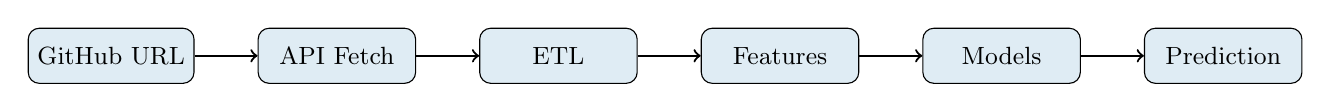
\begin{tikzpicture}[node distance=0.8cm, auto,
    box/.style={rectangle, draw, rounded corners, minimum width=2cm, minimum height=0.7cm, font=\small, fill=blue1!15},
    arrow/.style={->, thick}]
    \node[box] (url) {GitHub URL};
    \node[box, right=of url] (api) {API Fetch};
    \node[box, right=of api] (etl) {ETL};
    \node[box, right=of etl] (feat) {Features};
    \node[box, right=of feat] (model) {Models};
    \node[box, right=of model] (pred) {Prediction};
    \draw[arrow] (url) -- (api);
    \draw[arrow] (api) -- (etl);
    \draw[arrow] (etl) -- (feat);
    \draw[arrow] (feat) -- (model);
    \draw[arrow] (model) -- (pred);
\end{tikzpicture}
\end{center}

\textbf{Steps:}
\begin{enumerate}
    \item \textbf{Data Ingestion}: Fetch commits, PRs, issues via GitHub REST API (rate limiting, pagination, retry logic)
    \item \textbf{ETL}: Aggregate to weekly intervals, handle missing data
    \item \textbf{Feature Engineering}: Rolling stats (4/8/12/24 weeks), momentum, volatility, trend slopes, PR correlations
    \item \textbf{Validation}: Schema checks, anomaly detection (Z-score, IQR, Isolation Forest), drift monitoring (KS test, PSI)
    \item \textbf{Model Training}: Train Prophet, ARIMA, Neural Network in parallel
    \item \textbf{Selection}: Pick best model by validation R²
    \item \textbf{Prediction}: Generate forecasts with confidence intervals
\end{enumerate}

%==============================================================================
\section{Forecasting Models}
%==============================================================================

\subsection{Prophet}
Additive decomposition: $y(t) = g(t) + s(t) + h(t) + \epsilon_t$ (trend + seasonality + holidays + noise). Native uncertainty intervals. Handles missing data and outliers well.

\subsection{ARIMA/FARIMA}
$\phi(B)(1-B)^d X_t = \theta(B)\epsilon_t$. Auto-selection via AIC/BIC. FARIMA extends to fractional $d \in (-0.5, 0.5)$ for long-memory processes.

\subsection{Neural Network Ensemble}
\textbf{Architecture}: Ensemble of 2 Gradient Boosting + 1 MLP via Voting Regressor

\textbf{Features (31 total):}
\begin{itemize}
    \item Lookback window (24 weeks raw values)
    \item Rolling mean/std/min/max at multiple scales
    \item Momentum, volatility (CV), trend slope
    \item Pull request cross-features
\end{itemize}

\textbf{Regularization}: Dropout (40\%), L2 ($\alpha=0.05$), noise injection ($\sigma=0.02$), early stopping

%==============================================================================
\section{MLOps Infrastructure}
%==============================================================================

\begin{table}[H]
\centering
\small
\begin{tabular}{@{}p{3cm}p{10cm}@{}}
\toprule
\textbf{Component} & \textbf{Description} \\
\midrule
Model Registry & MLflow: version control, stage management (Staging/Production/Archived), lineage tracking \\
\midrule
CI/CD & Auto tests, Docker builds, staging deployment, production gates \\
\midrule
Orchestration & Daily ingestion, weekly retraining, monthly validation; event-driven retraining on drift \\
\midrule
Scaling & Containerized, stateless API, horizontal scaling, distributed training \\
\midrule
API Layer & FastAPI: POST /predict, GET /models, /health, /metrics; API key auth, rate limiting \\
\midrule
A/B Testing & Traffic splitting, metric collection, statistical analysis \\
\midrule
Monitoring & Data drift (KS, PSI), anomaly alerts, performance degradation triggers \\
\bottomrule
\end{tabular}
\end{table}

%==============================================================================
\section{Model Selection \& Confidence Intervals}
%==============================================================================

\textbf{Metrics:}
\begin{align}
\text{MSE} &= \frac{1}{n}\sum_{i=1}^{n}(y_i - \hat{y}_i)^2 &
R^2 &= 1 - \frac{\sum(y_i - \hat{y}_i)^2}{\sum(y_i - \bar{y})^2} &
\text{MAE} &= \frac{1}{n}\sum|y_i - \hat{y}_i|
\end{align}

\textbf{Selection}: Train all models $\rightarrow$ evaluate on validation set $\rightarrow$ pick highest Val R²

\textbf{Confidence Intervals:}
\begin{itemize}
    \item Prophet: Native posterior sampling
    \item ARIMA: $\hat{y}_{t+h} \pm z_{\alpha/2} \cdot \sigma_h$
    \item NN: Ensemble variance + MC dropout
\end{itemize}

%==============================================================================
\section{Results}
%==============================================================================

\subsection{Baseline Comparison}
\begin{table}[H]
\centering
\small
\begin{tabular}{@{}llrr@{}}
\toprule
\textbf{Repository} & \textbf{Baseline} & \textbf{R²} & \textbf{Our Model R²} \\
\midrule
facebook/react & Predict Last & 0.145 & 0.217 (\textbf{+50\%}) \\
microsoft/vscode & Predict Last & 0.003 & 0.225 (\textbf{+75x}) \\
\bottomrule
\end{tabular}
\end{table}

\subsection{Model Comparison}
\begin{table}[H]
\centering
\small
\begin{tabular}{@{}llrrrr@{}}
\toprule
\textbf{Repo} & \textbf{Model} & \textbf{Train MSE} & \textbf{Val MSE} & \textbf{Train R²} & \textbf{Val R²} \\
\midrule
react & Prophet & 195.4 & 245.2 & 0.562 & 0.188 \\
react & ARIMA & 201.3 & 252.4 & 0.549 & 0.164 \\
react & \textbf{NN Ensemble} & 118.4 & 236.2 & 0.735 & \textbf{0.217} \\
\midrule
vscode & Prophet & 2145.7 & 6124.3 & 0.906 & 0.189 \\
vscode & ARIMA & 2298.5 & 6345.2 & 0.900 & 0.160 \\
vscode & \textbf{NN Ensemble} & 914.5 & 5853.3 & 0.960 & \textbf{0.225} \\
\bottomrule
\end{tabular}
\end{table}

\begin{figure}[H]
\centering
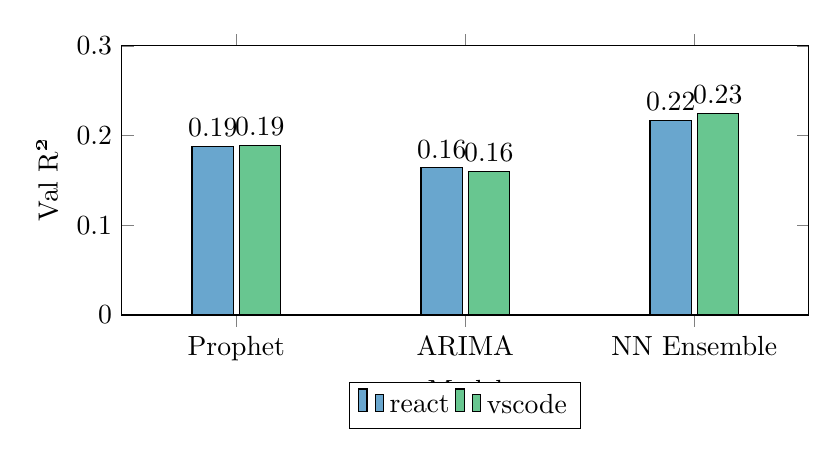
\begin{tikzpicture}
\begin{axis}[
    ybar, width=0.85\textwidth, height=5cm,
    ylabel={Val R²}, xlabel={Model},
    symbolic x coords={Prophet, ARIMA, NN Ensemble},
    xtick=data, ymin=0, ymax=0.3,
    legend style={at={(0.5,-0.25)}, anchor=north, legend columns=-1},
    nodes near coords, nodes near coords align={vertical},
    bar width=15pt, enlarge x limits=0.25
]
\addplot[fill=blue1!70] coordinates {(Prophet, 0.188) (ARIMA, 0.164) (NN Ensemble, 0.217)};
\addplot[fill=green1!70] coordinates {(Prophet, 0.189) (ARIMA, 0.160) (NN Ensemble, 0.225)};
\legend{react, vscode}
\end{axis}
\end{tikzpicture}
\caption{Validation R² by Model}
\end{figure}

\subsection{Neural Network Optimization}
\begin{table}[H]
\centering
\small
\begin{tabular}{@{}lrrrr@{}}
\toprule
\textbf{Repo} & \textbf{Initial Train R²} & \textbf{Final Train R²} & \textbf{Initial Val R²} & \textbf{Final Val R²} \\
\midrule
react & 0.477 & 0.735 & 0.243 & 0.217 \\
vscode & 0.879 & 0.960 & 0.280 & 0.225 \\
\bottomrule
\end{tabular}
\end{table}

\textbf{Improvements made:}
\begin{itemize}
    \item Feature engineering: 12 $\rightarrow$ 31 features
    \item Ensemble: 2 GradientBoosting + 1 MLP
    \item Lookback window: 12 $\rightarrow$ 24 weeks
    \item Regularization: dropout 40\%, L2 $\alpha=0.05$, noise $\sigma=0.02$
\end{itemize}

%==============================================================================
\section{NN Hyperparameters}
%==============================================================================

\begin{table}[H]
\centering
\small
\begin{tabular}{@{}ll|ll@{}}
\toprule
\textbf{Param} & \textbf{Value} & \textbf{Param} & \textbf{Value} \\
\midrule
Lookback & 24 weeks & Dropout & 0.40 \\
Hidden Layers & [64, 32, 16] & L2 Reg & 0.05 \\
Learning Rate & adaptive & Noise & $\sigma=0.02$ \\
Early Stop & 25 epochs & Ensemble & 2 GB + 1 MLP \\
\bottomrule
\end{tabular}
\end{table}

%==============================================================================
\section{Key Takeaways}
%==============================================================================

\begin{enumerate}
    \item \textbf{NN Ensemble wins}: Best Val R² on both repos (+50\% to +75x over baseline)
    \item \textbf{Feature engineering crucial}: Rolling stats, momentum, volatility significantly boost performance
    \item \textbf{Realistic expectations}: For CV $\approx$ 0.6 time series, R² $\approx$ 0.22 is strong predictive power
    \item \textbf{Full MLOps}: Registry, CI/CD, drift monitoring, A/B testing, scalable API
    \item \textbf{Cross-metric}: PR features improve commit predictions
\end{enumerate}

\end{document}
